%================================================
\setcounter{framenumber}{0}
%\renewcommand{\mydate}{{2026年03月03日\ 第一次课}}
%================================================
%================================================
\section{向量}
\title{第一章 \quad 向量}
\author{}
\date{}
%================================================
%================================================
\frame{\titlepage}
%================================================
%================================================


\subsection{向量及其运算}


\subsubsection{什么是向量}
\begin{frame}\frametitle{什么是向量}
我们初中学习过一些物理量包括\blue{速度}、\blue{位移}、\blue{力}等等.\\[3mm]

\includegraphics[scale=0.3]{pic/Velocity.jpg}
\quad

\includegraphics[scale=0.2]{pic/AB.png}
\quad
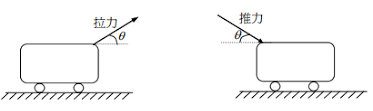
\includegraphics[scale=0.5]{pic/Force.png}
\ \\[10mm]
\pp
数学上的抽象总结:
\begin{center}
\framebox(300,50){ \LARGE \blue{向量} = 既有\underline{大小},又有\underline{方向}的量.}
\end{center}
\end{frame}





%\subsubsection{什么是向量}
%\begin{frame}\frametitle{向量的表达、模长、夹角}
%\begin{enumerate}
%	\item \blue{表达方式}:$\overset{\longrightarrow}{AB}$, $\vec{a}$, $\vec{b}$, $\vec{c}$, $\bf{a}$, $\bf{b}$, $\bf{c}$.
%	\item \blue{模长}: 向量的长度. 向量$\vec{a}$的模长记为$|\vec{a}|$.
%	\begin{itemize}
%		\item \blue{零向量}:$|\vec{a}|=0$. \blue{规定}任意方向都为零向量的方向.
%		\item \blue{单位向量}:$|\vec{a}|=1$.
%	\end{itemize}
%	\item \blue{相等}:大小相同,方向相同. 记为: $\vec{a}=\vec{b}$.\\
%\begin{equation*}
%\begin{tikzpicture}[scale=1]
%\tikzmath{\r=3;};
%\tikzmath{\R=5.5;};
%\coordinate (O) at (0,0);
%\coordinate (A) at (1,2);
%\coordinate (B) at (2,1);
%\draw[->,thick,blue](O)--(A) node[pos=.5,sloped,above] {$\vec{a}$};
%\draw[->,thick,red](O)--(B) node[pos=.5,sloped,above] {$\vec{b}$};
%\pp
%\coordinate (o) at (0+\r,0);
%\coordinate (a) at (1+\r,2);
%\coordinate (b) at (0.5+\r,1);
%\draw[->,thick,blue](o)--(a) node[pos=.5,sloped,above] {$\vec{a}$};
%\draw[->,red](o)--(b) node[pos=.5,sloped,above] {$\vec{b}$};
%\pp
%\coordinate (oo) at (0+\R,0);
%\coordinate (cc) at (1+\R,0);
%\coordinate (aa) at (1+\R,2);
%\coordinate (bb) at (2+\R,2);
%\draw[->,thick,blue](oo)--(aa) node[pos=.5,sloped,above] {$\vec{a}$};
%\draw[->,red](cc)--(bb) node[pos=.5,sloped,above] {$\vec{b}$};
%\draw[dotted](oo)--(cc);
%\draw[dotted](bb)--(aa);
%\end{tikzpicture}
%\end{equation*}
%	\item \blue{反向量}(\blue{负向量}):大小相同,方向相反. 记为 $-\vec{a}$.
%	\item \blue{夹角} 
\includegraphics[scale=0.2]{angle.png} $0\leq \theta \leq \pi$.
%	\begin{itemize}
%		\item \blue{平行}($\theta=0$或$\pi$). 特别地,零向量与任意向量平行.
%		\item \blue{垂直}或\blue{正交}($\theta=\frac\pi2$).
%	\end{itemize}
%\end{enumerate}
%\end{frame}





\subsubsection{向量加法}
\begin{frame}\frametitle{向量加法}
\begin{center}
速度,力的合成 \quad $\xRightarrow{\text{用数学语言抽象化}}$ \quad 向量的加法
\end{center}
\pp
\begin{definition}[向量的加法---平行四边形法则或者三角形法则]
\begin{equation*}
\begin{tikzpicture}[scale=1]
\tikzmath{\r=4;};
\coordinate (O) at (0,0);
\coordinate (A) at (1,2);
\coordinate (B) at (1.5,-0.5);
\coordinate (C) at (2.5,1.5);

\coordinate (o) at (0+\r,0);
\coordinate (a) at (1+\r,2);
\coordinate (b) at (1.5+\r,-0.5);
\coordinate (c) at (2.5+\r,1.5);

\draw[->,thick,blue](O)--(A) node[pos=.5,sloped,above] {$\vec{a}$};
\draw[->,thick,red](O)--(B) node[pos=.5,sloped,above] {$\vec{b}$};
\pp
\draw[dotted](A)--(C);
\draw[dotted](B)--(C);
\pp
\draw[->,thick,purple](O)--(C) node[pos=.5,sloped,above] {$\vec{a}+\vec{b}$};
\pp
\draw[->,thick,blue](o)--(a) node[pos=.5,sloped,above] {$\vec{a}$};
\pp
\draw[->,thick,red](a)--(c) node[pos=.5,sloped,above] {$\vec{b}$};
\pp
\draw[->,thick,purple](o)--(c) node[pos=.5,sloped,above] {$\vec{a}+\vec{b}$};
\end{tikzpicture}
\end{equation*}
\end{definition}
\end{frame}





\subsubsection{向量加法的基本性质}
\begin{frame}\frametitle{向量加法的基本性质}
\begin{proposition}[向量加法的基本性质]
\pp
\begin{enumerate}
\item 加法交换律: $\vec{a}+\vec{b}=\vec{b}+\vec{a}$;
\pp
\item 加法结合律: $\vec{a}+(\vec{b}+\vec{c})=(\vec{a}+\vec{b})+\vec{c}$;
\pp
\item 存在零元: $\vec{a}+\vec{0}=\vec{a}=\vec{0}+\vec{a}$;
\pp
\item 存在负元: $\vec{a}+(-\vec{a})=\vec{0}=(-\vec{a})+\vec{a}$;
\pp
\end{enumerate}
\end{proposition}
\end{frame}



\subsubsection{向量减法}
\begin{frame}\frametitle{向量减法}
\begin{definition}[向量的减法]
\[\vec{a}-\vec{b}:=\vec{a}+(-\vec{b}).\]
%\footnote{注: 先定义负元,后定义减法.}
\end{definition}

\pp

\begin{equation*}
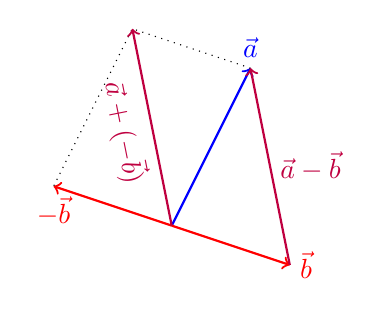
\begin{tikzpicture}[scale=1]
\coordinate (O) at (0,0);
\coordinate (A) at (1,2);
\coordinate (B) at (1.5,-0.5);
\coordinate (b) at (-1.5,0.5);
\coordinate (C) at (-0.5,2.5);
\pp
\draw[->,thick,blue](O)--(A) node[pos=1,above] {$\vec{a}$};
\draw[->,thick,red](O)--(B) node[pos=1,right] {$\vec{b}$};
\pp
\draw[->,thick,red](O)--(b) node[pos=1,below] {$-\vec{b}$};
\pp
\draw[dotted](A)--(C)--(b);
\pp
\draw[->,thick,purple](O)--(C) node[pos=0.5,sloped,below] {$\vec{a}+(-\vec{b})$};
\pp
\draw[->,thick,purple](B)--(A) node[pos=0.5,right] {$\vec{a}-\vec{b}$};
\end{tikzpicture}
\end{equation*}


\end{frame}





\subsubsection{向量的数乘}
\begin{frame}\frametitle{向量的数乘}
\begin{equation*}
\begin{tikzpicture}[scale=1]
\coordinate (O) at (0,0);\draw [fill] (O) circle [radius=0.03];
\coordinate (A) at (1,0);
\coordinate (05A) at (0.5*1,0);
\coordinate (2A) at (2*1,0);
\coordinate (mA) at (-1*1,0);
\coordinate (m15A) at (-1.5*1,0);
\coordinate (B) at (-1,1);
\coordinate (mpiB) at (3.14,-3.14);
\coordinate (eB) at (-2.718,2.718);
\draw[->,thick,blue](O)--(A) node[pos=1,sloped,below] {$\vec{a}$};
\pp
\draw[->,red](O)--(05A) node[pos=1,sloped,above] {$0.5\vec{a}$};
\pp
\draw[->,red](O)--(2A) node[pos=1,sloped,above] {$2\vec{a}$};
\pp
\draw[->,thick,green](O)--(mA) node[pos=1,sloped,below] {$-\vec{a}$};
\pp
\draw[->,purple](O)--(m15A) node[pos=1.2,sloped,above] {$-1.5\vec{a}$};
\pp
\draw[->,thick,blue](O)--(B) node[pos=1,above] {$\vec{b}$};
\draw[->,black](O)--(mpiB) node[pos=1,below] {$-\pi\vec{b}$};
\draw[->,black](O)--(eB) node[pos=1,above] {$e\vec{b}$};
\pp
\end{tikzpicture}
\end{equation*}
\end{frame}






\begin{frame}\frametitle{向量的数乘}
\begin{definition}[向量的数乘] 令$\vec{a}$为一向量, $\lambda$为一实数.\\
$\bullet$ 若$\lambda\geq0$,则$\lambda \vec{a}$定义为长度为$\lambda |\vec{a}|$且方向与$\vec{a}$相同的向量.\\
\pp
$\bullet$ 若$\lambda<0$,则$\lambda \vec{a}$定义为长度为$-\lambda |\vec{a}|$且方向与$\vec{a}$相反的向量.
\end{definition}
\pp

\textbf{记号}: 若 $\vec{a}\neq\vec{0}$,则记 $\blue{\vec{a}^0}:=\frac{1}{|\vec{a}|}\vec{a}$. 即, $\vec{a}^0$为方向与$\vec{a}$相同的\blue{单位向量}.
\pp

注：\blue{零向量}:$|\vec{a}|=0$. \blue{规定}任意方向都为零向量的方向.
\end{frame}





\subsubsection{向量数乘的基本性质}
\begin{frame}\frametitle{向量数乘的基本性质}
\begin{proposition}[向量数乘的基本性质]
\pp
\begin{enumerate}\setcounter{enumi}{4}
\item 数乘单位元: $1\vec{a} = \vec{a}$;
\pp
\item 数乘结合律: $\lambda(\mu \vec{a})=(\lambda \mu)\vec{a}$;
\pp
\item 左分配律: $(\lambda+\mu)\vec{a}=\lambda \vec{a} + \mu \vec{a}$;
\pp
\item 右分配律: $\lambda (\vec{a}+\vec{b}) =\lambda \vec{a} + \lambda \vec{b}$;
\end{enumerate}
\end{proposition}
\end{frame}





\subsubsection{线性运算}
\begin{frame}\frametitle{线性运算}
\begin{definition}[线性运算]
向量的\blue{加法}和\blue{数乘}运算统称为向量的\blue{线性运算}.
\end{definition}
\pp
\begin{proposition}[向量线性运算的八条基本性质]
\begin{enumerate}
\item 加法交换律: $\vec{a}+\vec{b}=\vec{b}+\vec{a}$;
\item 加法结合律: $\vec{a}+(\vec{b}+\vec{c})=(\vec{a}+\vec{b})+\vec{c}$;
\item 存在零元: $\vec{a}+\vec{0}=\vec{a}=\vec{0}+\vec{a}$;
\item 存在负元: $\vec{a}+(-\vec{a})=\vec{0}=(-\vec{a})+\vec{a}$;
\item 数乘单位元: $1\vec{a} = \vec{a}$;
\item 数乘结合律: $\lambda(\mu \vec{a})=(\lambda \mu)\vec{a}$;
\item 左分配律: $(\lambda+\mu)\vec{a}=\lambda \vec{a} + \mu \vec{a}$;
\item 右分配律: $\lambda (\vec{a}+\vec{b}) =\lambda \vec{a} + \lambda \vec{b}$;
\end{enumerate}
\end{proposition}
\pp
注：我们将通过这八条性质来公理化地定义一般的\blue{线性空间}或\blue{向量空间} (书本第五章,课件第六章).
\end{frame}





\subsection{向量线性相关性}





\subsubsection{线性组合}
\begin{frame}\frametitle{线性组合}
\begin{definition}[线性组合]
设 $\vec{a}_1$, $\vec{a}_2$, $\cdots$, $\vec{a}_m$  为一组向量, $\lambda_1$, $\lambda_2$, $\cdots$, $\lambda_m$ 为一组实数. 称向量
\[\lambda_1\vec{a}_1 + \lambda_2\vec{a}_2 + \cdots + \lambda_m\vec{a}_m\]
为向量 $\vec{a}_1$, $\vec{a}_2$, $\cdots$, $\vec{a}_m$ 的\blue{线性组合}.
\end{definition}
\pp
也就是说,一组向量的线性组合就是从这组向量出发通过线性运算能够获得的向量.
\pp
\begin{equation*}
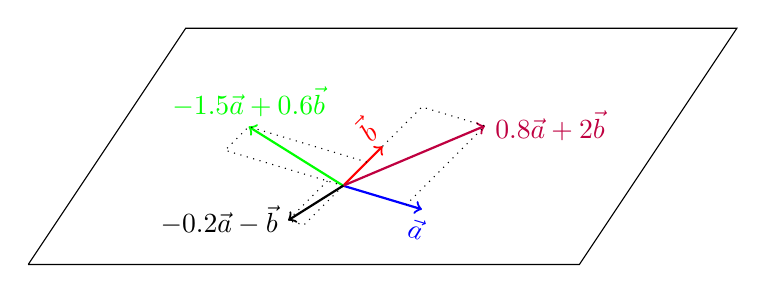
\begin{tikzpicture}[scale=1]
\coordinate (O) at (0,0);
\coordinate (A) at (1,-0.3);
\coordinate (B) at (0.5,0.5);
%---
\coordinate (08A) at (0.8,-0.24);
\coordinate (2B) at (1,1);
\coordinate (C1) at (1.8,0.76);   %0.8*(A)+2*(B);
%---
\coordinate (m15A) at (-1.5,0.45);
\coordinate (06B) at (0.3,0.3);
\coordinate (C2) at (-1.2,0.75);   %0.8*(A)+2*(B);
%---
\coordinate (m02A) at (-0.2,0.06);
\coordinate (mB) at (-0.5,-0.5);
\coordinate (C3) at (-0.7,-0.44);   %0.8*(A)+2*(B);
%---
\coordinate (D) at (-0.5,2.5);
\pp
\draw (-4,-1)--(-2,2)--(5,2)--(3,-1)--(-4,-1);
\draw[->,thick,blue](O)--(A) node[pos=1,sloped,below] {$\vec{a}$};
\draw[->,thick,red](O)--(B) node[pos=1,sloped,above] {$\vec{b}$};
\pp
\draw[->,thick,purple](O)--(C1) node[pos=1,right] {$0.8\vec{a}+2\vec{b}$};
\draw[dotted](B)--(2B)--(C1)--(08A);
\pp
\draw[->,thick,green](O)--(C2) node[pos=1,above] {$-1.5\vec{a}+0.6\vec{b}$};
\draw[dotted](06B)--(C2)--(m15A)--(O);
\pp
\draw[->,thick,black](O)--(C3) node[pos=1,left] {$-0.2\vec{a}-\vec{b}$};
\draw[dotted](m02A)--(C3)--(mB)--(O);
\end{tikzpicture}
\end{equation*}


\end{frame}


\subsubsection{线性组合的几何解释}
\begin{frame}\frametitle{线性组合的几何解释}

\begin{center}\blue{\framebox(300,50){
$\xymatrix@R=0mm@C=3cm{
\text{空间} \ar@{<->}[r]_-{\text{固定一个点$O$(原点)}}^-{1:1}& \text{全体向量集}\\
P \ar@{|->}[r] & \overset{\longrightarrow}{OP}\\
}$}}
\end{center}
\pp
\bigskip

\begin{enumerate}
\item 设 $\vec{a}$为一个非零向量。则
\begin{center}
过原点与 $\vec{a}$ 平行的\blue{直线} \quad $\xleftrightarrow{\quad 1:1 \quad}$ \quad $\vec{a}$的全体线性组合.
\end{center}
\pp
\bigskip


\item 设$\vec{a},\vec{b}$不平行(不共线). 则
\begin{center}
过原点与 $\vec{a}$ 和 $\vec{b}$ 平行的\blue{平面} \quad $\xleftrightarrow{\quad 1:1 \quad}$\quad  $\vec{a},\vec{b}$ 的全体线性组合.
\end{center}
\end{enumerate}

\pp
\bigskip

\red{这就是线性组合的威力:用少数几个向量表示特定子空间!}

\end{frame}








\subsubsection{线性相关与线性无关}
\begin{frame}\frametitle{线性相关与线性无关}
\begin{definition}[线性相关,线性无关] 给定一组向量 $\vec{a}_1$, $\vec{a}_2$, $\cdots$, $\vec{a}_m$.
\begin{itemize}
\item 如果存在一组不全为零的实数 $\lambda_1$, $\lambda_2$, $\cdots$, $\lambda_m$ 使得
\[\lambda_1\vec{a}_1 + \lambda_2\vec{a}_2 + \cdots + \lambda_m\vec{a}_m=\vec{0},\]
则称向量组$\vec{a}_1$, $\vec{a}_2$, $\cdots$, $\vec{a}_m$\blue{线性相关}.
\pp
\item 反之,若对任意一组不全为零的实数$\lambda_1$, $\lambda_2$, $\cdots$, $\lambda_m$都有
\[\lambda_1\vec{a}_1 + \lambda_2\vec{a}_2 + \cdots + \lambda_m\vec{a}_m\neq \vec{0},\]
则称向量组 $\vec{a}_1$, $\vec{a}_2$, $\cdots$, $\vec{a}_m$的\blue{线性无关}.
\end{itemize}
\end{definition}
\pp
\bigskip

特别地，设 $\vec{a}_1$, $\vec{a}_2$, $\cdots$, $\vec{a}_m$\blue{线性无关}. 若 $\lambda_1\vec{a}_1 + \lambda_2\vec{a}_2 + \cdots + \lambda_m\vec{a}_m= \vec{0}$, 则
$\lambda_1=\lambda_2= \cdots=\lambda_m=0$.

\pp
\bigskip

%\begin{example}
%向量组 \(\vec{a} = (1, 2, 3)\)，\(\vec{b} = (2, 3, 4)\)，\(\vec{c} = (3, 5, 7)\) 线性相关. 这是由于 \( \vec{a} +  \vec{b} - \vec{c} = \vec{0}\).
%\end{example}
%
%
%\begin{example}
%向量组 \(\vec{a} = (1, 0, 0)\)，\(\vec{b} = (0, 1, 0)\)，\(\vec{c} = (0, 0, 1)\) 线性无关. 假如线性相关, 则存在不全为零的实数 \(\lambda_1, \lambda_2, \lambda_3\) 使得
%\[\lambda_1 \vec{a} + \lambda_2 \vec{b} + \lambda_3 \vec{c} = \vec{0}\]
%即,
%   \[(\lambda_1, \lambda_2, \lambda_3) = (0, 0, 0)\]
%\end{example}



\begin{example}证明向量组$\vec{e}_1=\vec{a}+\vec{b}+\vec{c}$, $\vec{e}_2=\vec{a}-\vec{b}-\vec{c}$, $\vec{e}_3=\vec{a}+2\vec{b}+2\vec{c}$线性相关。
\end{example}

\pp

\red{$3\vec{e}_1 - \vec{e}_2 - 2\vec{e}_3 =\vec{0}$ 或 $\vec{e}_2 = 3\vec{e}_1-2\vec{e}_3$.}
\end{frame}





\subsubsection{线性相关的几何解释}
\begin{frame}\frametitle{线性相关的几何解释}
\begin{enumerate}
\item 一个向量$\vec{a}$线性相关 $\iff$ $\vec{a}=\vec0$;
\pp
\bigskip

\item 两个向量$\vec{a},\vec{b}$线性相关 $\iff$ $\vec{a}$与$\vec{b}$平行(共线);
\pp
\bigskip

\item 三个向量$\vec{a},\vec{b},\vec{c}$线性相关 $\iff$ $\vec{a},\vec{b},\vec{c}$共面;
\pp
\bigskip

\item 四个及四个以上的向量一定线性相关.
\end{enumerate}
\end{frame}








\subsection{坐标系、坐标与坐标变换}


\subsubsection{仿射坐标系}
\begin{frame}\frametitle{仿射坐标系}
为了推广笛卡尔坐标系到坐标轴不相互垂直的情形,
\begin{equation*}
\begin{tikzpicture}[scale=1]
\coordinate (o) at (0,0);
\coordinate (y) at (1,0);
\coordinate (x) at (-0.5,-0.5);
\coordinate (z) at (0,1);
\draw[->,thick,black](o)--(x) node[pos=1,below] {$x$};
\draw[->,thick,black](o)--(y) node[pos=1,right] {$y$};
\draw[->,thick,black](o)--(z) node[pos=1,above] {$z$};
\tkzMarkRightAngle(x,o,y)
\tkzMarkRightAngle(y,o,z)
\tkzMarkRightAngle(z,o,x)

\coordinate (O) at (4,0);
\node [below left] at (O) {$O$};
\coordinate (X) at (6,-1);
\coordinate (Y) at (5,0.5);
\coordinate (Z) at (3.5,1);
\draw[->,thick,black](O)--(X) node[pos=1,right] {$\vec{e}_1$};
\draw[->,thick,black](O)--(Y) node[pos=1,right] {$\vec{e}_2$};
\draw[->,thick,black](O)--(Z) node[pos=1,above] {$\vec{e}_3$};
\end{tikzpicture}
\end{equation*}
\pp
我们需要引入向量的基本定理.
\begin{theorem}[向量的基本定理]
设$\vec{e}_1$, $\vec{e}_2$, $\vec{e}_3$ 为空间中的三个不共面的向量, 则对每个向量$\vec{a}$都\blue{存在唯一}的三元有序实数组$(x_1,x_2,x_3)$, 使得
\[\vec{a} = x_1\vec{e}_1 + x_2\vec{e}_2 + x_3\vec{e}_3.\]
\end{theorem}
\end{frame}





\begin{frame}\frametitle{仿射坐标系}
\begin{definition}[基、坐标]
称不共面的三个向量$\vec{e}_1,\vec{e}_2,\vec{e}_3$为一组\blue{基}. 若
\[\vec{a} = x_1\vec{e}_1 + x_2\vec{e}_2 + x_3\vec{e}_3,\]
则称$(x_1,x_2,x_3)$为向量$\vec{a}$在基$\vec{e}_1,\vec{e}_2,\vec{e}_3$下的\blue{(仿射)坐标}.
\end{definition}
\pp
\begin{equation*}
\boxed{\blue{\text{仿射坐标系}}=\text{点} O  + \text{基} \vec{e}_1,\vec{e}_2,\vec{e}_3 \qquad \text{记作} \blue{[O;\vec{e}_1,\vec{e}_2,\vec{e}_3]}.}
\end{equation*}
\pp
%\blue{坐标原点}, \blue{坐标向量}, \blue{$x$轴}, \blue{$y$轴}, \blue{$z$轴}, \blue{坐标平面$Oxy$}, \blue{$Oyz$}, \blue{$Ozx$}.\\[2mm]
\begin{corollary}[一一对应]
若给定仿射坐标系 $[O;\vec{e}_1,\vec{e}_2,\vec{e}_3]$,则有如下一一对应
\begin{center}\blue{\framebox(300,50){
$\xymatrix@R=0mm{
\text{空间} \ar@{<->}[r]^-{1:1}& \text{全体向量集} \ar@{<->}[r]^-{1:1} & \mathbb R^3=\mathbb R\times \mathbb R \times \mathbb R \\
P \ar@{|->}[r] & \overset{\longrightarrow}{OP} \ar@{|->}[r] & \text{坐标}(x_1,x_2,x_3) \\
}$}}
\end{center}
\end{corollary}
\end{frame}





\subsubsection{向量的坐标运算}
\begin{frame}\frametitle{向量的坐标运算}
给定仿射坐标系 $[O;\vec{e}_1,\vec{e}_2,\vec{e}_3]$, 我们用$(x_1,x_2,x_3)$表示向量$x_1\vec{e}_1+x_2\vec{e}_2+x_3\vec{e}_3$.
\pp 则我们有
\begin{proposition}
$\bullet$ $(x_1,x_2,x_3) + (y_1,y_2,y_3) = (x_1+y_1,x_2+y_2,x_3+y_3)$;\\
\pp
$\bullet$ $\lambda(x_1,x_2,x_3) = (\lambda x_1,\lambda x_2,\lambda x_3)$.
\end{proposition}

\forppt{
\red{
\begin{equation*}
\begin{split}
(x_1,x_2,x_3) + (y_1,y_2,y_3) & := (x_1\vec{e}_1+x_2\vec{e}_2+x_3\vec{e}_3) + (y_1\vec{e}_1+y_2\vec{e}_2+y_3\vec{e}_3) \\
& = (x_1+y_1)\vec{e}_1 +(x_2+y_2)\vec{e}_2 +(x_3+y_3)\vec{e}_3 \\
& =: (x_1+y_1,x_2+y_2,x_3+y_3)\\
\lambda(x_1,x_2,x_3) & := \lambda (x_1\vec{e}_1+x_2\vec{e}_2+x_3\vec{e}_3) \\
& = \lambda x_1\vec{e}_1+\lambda x_2\vec{e}_2+\lambda x_3\vec{e}_3 \\
& =:  (\lambda x_1,\lambda x_2,\lambda x_3)\\
\end{split}
\end{equation*}
}}
\end{frame}








% ========== 2023年03月09号 第02次课 高维向量、数域、线性方程组 ==========




\subsubsection{坐标变换}
\begin{frame}\frametitle{坐标变换}
给定两个仿射坐标系 $[O;\vec{e}_1,\vec{e}_2,\vec{e}_3]$ 和 $[O';\vec{e}'_1,\vec{e}'_2,\vec{e}'_3]$.
\pp
\begin{question}
设空间中的点$P$在两个坐标系下的坐标分别为 $(x,y,z)$ 和 $(x',y',z')$. 求两个坐标之间的关系式？
\end{question}
\pp
为了回答这一问题，我们需要给出两个坐标系之间的位置关系:
\pp
\begin{itemize}
\item 设$O$在$[O';\vec{e}'_1,\vec{e}'_2,\vec{e}'_3]$下的坐标为$(x_0',y_0',z_0')$. 即
\[\overset{\longrightarrow}{O'O} = x'_0\vec{e}'_1+ y'_0\vec{e}'_2 + z'_0\vec{e}'_3.\]
\item \pp  设$\vec{e}_j$在基$\vec{e}'_1,\vec{e}'_2,\vec{e}'_3$下的坐标为$(a_{1j},a_{2j},a_{3j})$.即
\[ \vec{e}_j = a_{1j}\vec{e}'_1+ a_{2j}\vec{e}'_2 + a_{3j}\vec{e}'_3.\]
\end{itemize}
\pp
然后$P$在两个坐标系下的坐标之间的关系式可写为\footnote{后续,通过矩阵乘法可简化为 \blue{$X'=AX+X_0'$}.}：
\begin{equation*}
\blue{\boxed{
\begin{split}
x' &= a_{11}x+a_{12}y+a_{13}z+x_0'\\
y' &= a_{21}x+a_{22}y+a_{23}z+y_0'\\
z' &= a_{31}x+a_{32}y+a_{33}z+z_0'\\
\end{split}
}}\qquad
\pp  \red{pf: \overset{\longrightarrow}{O'P} = \overset{\longrightarrow}{O'O}+\overset{\longrightarrow}{OP}.}
\end{equation*}
\end{frame}




%\renewcommand{\mydate}{2025年2月27日\ 第二次课}

%\frame{\date{第二次课}\titlepage}


\subsection{复数与数域}





\subsubsection{复数}
\begin{frame}\frametitle{复数}
\begin{equation*}
\boxed{\xymatrix@R=4mm{
&\fbox{\text{\tiny 复数的代数表示}} &\sqrt{-1} \ar@<-1mm>[d]\\
z \ar@{}[r]|{=} & \underline{x} \ar@{}[r]|+ & \underline{i\ y}\\
&{\text{实部} \atop \mathrm{Re}z}\ar[u]&{\text{虚部}\atop \mathrm{Im}z}\ar[u]\\}}
\end{equation*}
\pp

\begin{columns}[c]
\column{5cm}
\boxed{\begin{tikzpicture}
\filldraw[black] (0,0) circle (2pt) node[below left]{$O$};
\filldraw[black] (2,1) circle (1pt) node[below]{};
\filldraw[black] (2,0) circle (1pt) node[below]{};
\filldraw[black] (0,1) circle (1pt) node[below]{};
\draw[black, thick,->]  (0,-0.5) -- (0,3) node[black,right]{虚轴};
\draw[black, thick,->]  (-0.5,0) -- (4,0) node[black,right]{实轴};
\draw[black, thick,dotted]  (2,1) -- (2,0) node[black,below]{$x$};
\draw[black, thick,dotted]  (2,1) -- (0,1) node[black,left]{$y$};
\draw[black, thick,->]  (0,0) -- (2,1) node[black,right]{${P(x,y) \atop z=x+iy}$};
\node[black] at (3.5,2.5){复平面};
\node[black] at (2,3.2){\fbox{\tiny 复数的几何表示}};
\node[black] at (0.8,0.2){$\theta$};
\node[black] at (1,0.7){$r$};
\draw[black, thick,-]  (0.44,0) -- (0.4,0.2);
\end{tikzpicture}}
\column{5cm}
\pp
\begin{itemize}
\item \blue{模长}:  $|z|:=|\overset{\longrightarrow}{OP}|=\sqrt{x^2+y^2}$;
\item \blue{辐角}: 实轴沿逆时针方向旋转到$\overset{\longrightarrow}{OP}$的角度.
\item \blue{共轭}: $\overline{z}:=x-iy$.
\item \blue{三角表示}:\\ $z=r(\cos\theta+i\sin\theta)$.
\end{itemize}
\end{columns}
\end{frame}







\subsubsection{数域}
\begin{frame}\frametitle{数域}
复数域的任意子集称为\blue{数集}. 例如: $\mathbb N$, $\mathbb Z$, $\mathbb Q$, $\mathbb R$,$\mathbb C$, $\cdots$.
\pp
\begin{definition} 若数集$\mathbb F$至少包含两元素,且关于数的{\bf 加减乘除封闭},则称$\mathbb F$为\blue{数域}.
\end{definition}
\pp
\begin{example}[本课程中最常用的域]
有理数集$\mathbb Q$,实数集$\mathbb R$,和复数集$\mathbb C$均为数域.
\end{example}
注:$\mathbb N$, $\mathbb Z$不为数域.
\pp

\blue{为什么需要数域概念?}
\begin{itemize}
\item 向量的坐标可以是实数,也可以是复数;
\item 统一的数域概念让我们可以同时处理实向量和复向量;
\item 后面的线性空间理论建立在任意数域上.
\end{itemize}

\pp
\yang{注:\begin{enumerate}
\item $\mathbb Q[\sqrt{2}]=\{a+b\sqrt2\mid a,b\in\mathbb Q\}$也是数域,但本课程不作要求.
\item $\mathbb Q$ 为最小的数域. 即,若$\mathbb F$为数域,则$\mathbb Q\subseteq \mathbb F$.
\end{enumerate}}
\end{frame}





\subsection{数组向量}


\subsubsection{高维数组向量的定义}
\begin{frame}\frametitle{高维数组向量的定义}
设$\mathbb F$为数域, $n$为正整数.
\pp
\begin{definition}我们称一个由$n$个$\mathbb F$上的数$a_1,a_2,\cdots,a_n$组成的有序数组
\[\vec{a} := (a_1,\cdots,a_n)\]
为\blue{数域$\mathbb F$上的一个$n$维数组向量}.其中$a_i$称为$\vec{a}$的\blue{第$i$个分量}. 数域$\mathbb F$上$n$维数组向量全体记为 \blue{$\mathbb F^n$}.
\end{definition}
\pp
记法:
\begin{equation*}
\blue{\text{行向量:\ }} \vec{a} = (a_1,\cdots,a_n)\in \mathbb F^n \qquad \blue{\text{列向量:\ }} \vec{a}=\left(\begin{array}{c}a_1\\a_2\\\vdots\\a_n\\\end{array}\right)\in \mathbb F^n
\end{equation*}
\end{frame}




% ===== 新增:从三维到高维的过渡 =====
\subsubsection{从三维到高维}
\begin{frame}\frametitle{从三维到高维}
\begin{question}
三维空间中的向量有三个分量$(x,y,z)$. 那么四维、五维向量是什么?
\end{question}
\pp

\blue{例子1:时空向量(四维)}
\begin{itemize}
\item 相对论中,事件由时间和空间位置确定:$(t,x,y,z)$
\item 这是一个\blue{四维向量}!
\end{itemize}
\pp

\blue{例子2:颜色向量(三维或四维)}
\begin{itemize}
\item RGB颜色模型:$(R,G,B)$ (红、绿、蓝三个分量)
\item RGBA颜色模型:$(R,G,B,A)$ (增加透明度分量)
\end{itemize}
\pp

\blue{例子3:学生成绩向量(n维)}
\begin{itemize}
\item 一个学生的成绩可以表示为:$(\text{数学},\text{物理},\text{化学},\text{英语},\cdots)$
\item 如果有$n$门课,就是一个\blue{$n$维向量}!
\end{itemize}
\pp

\bigskip

\begin{center}
\framebox{\blue{向量的维数 = 描述对象所需的独立参数个数 = 自由度}}
\end{center}
\end{frame}

\subsubsection{高维向量的应用}
\begin{frame}\frametitle{高维向量的应用}
\begin{example}[机器学习中的特征向量]
要识别一张图片是否包含猫,需要提取图片的特征:
\begin{itemize}
\item 颜色直方图(256维)
\item 边缘特征(128维)
\item 纹理特征(64维)
\item $\cdots$
\end{itemize}
\pp
最终得到一个\blue{几千维的向量}来表示这张图片!
\end{example}
\pp

\begin{example}[推荐系统中的用户向量]
一个用户对$n$部电影的评分可以表示为一个$n$维向量:
\[(r_1,r_2,\cdots,r_n)\]
其中$r_i$是用户对第$i$部电影的评分。
\end{example}

\end{frame}

\begin{frame}\frametitle{大模型中的高维向量}

\begin{example}[DeepSeek-V3]
设 $T$ 是 DeepSeek-V3 的 token 词表,  $|T|=129280$. \pp 词嵌入给每个 token 分配一个 7168 维向量：
\[E \colon  T \longrightarrow \mathbb R^{7168}.\]
\pp
为了储存映射 $E$, 我们需要
\[129208 \times 7168 = 926679040\]
个参数。
\pp
这约 9.27 亿个参数最初随机初始化, 之后与整个模型一起训练; 这些向量不是人工规定的,而是从大量语言数据中学习出来的.
\end{example}


\red{高维向量在现代科学和工程中无处不在!}

\end{frame}

% ===== 原有的高维数组向量定义(652-693行) =====




\subsubsection{高维数组向量的线性运算}
\begin{frame}\frametitle{高维数组向量的线性运算}
设 $\vec{a}=(a_1,\cdots,a_n)\in \mathbb F^n$, $\vec{b}=(b_1,\cdots,b_n)\in \mathbb F^n$, $\lambda\in \mathbb F$.
\begin{enumerate}[]
\item 加法: $\vec{a}+\vec{b}:=(a_1+b_1,a_2+b_2,\cdots,a_n+b_n)$.
\pp
\item 数乘: $\lambda \vec{a}:=(\lambda a_1,\lambda a_2,\cdots,\lambda a_n)$.
\pp
\item 零向量: $\vec{0}:=(0,\cdots,0)$.
\item 负向量: $-\vec{a}:=(-a_1,\cdots,-a_n)$.
\item 相等: $\vec{a}=\vec{b} \iff a_i=b_i \quad i=1,\cdots,n$.
\end{enumerate}
\pp
\blue{八条基本性质:}
\begin{enumerate}
\item 加法交换律: $\vec{a}+\vec{b}=\vec{b}+\vec{a}$;
\item 加法结合律: $\vec{a}+(\vec{b}+\vec{c})=(\vec{a}+\vec{b})+\vec{c}$;
\item 存在零元: $\vec{a}+\vec{0}=\vec{a}=\vec{0}+\vec{a}$;
\item 存在负元: $\vec{a}+(-\vec{a})=\vec{0}=(-\vec{a})+\vec{a}$;
\item 数乘单位元: $1\vec{a} = \vec{a}$;
\item 数乘结合律: $\lambda(\mu \vec{a})=(\lambda \mu)\vec{a}$;
\item 左分配律: $(\lambda+\mu)\vec{a}=\lambda \vec{a} + \mu \vec{a}$;
\item 右分配律: $\lambda (\vec{a}+\vec{b}) =\lambda \vec{a} + \lambda \vec{b}$;
\end{enumerate}
\end{frame}




\subsubsection{线性相关(高维数组向量)}
\begin{frame}\frametitle{线性相关(高维数组向量)}
设$\vec{a}_1,\vec{a}_2,\cdots,\vec{a}_m\in \mathbb F^n$,  $\lambda_1,\lambda_2,\cdots,\lambda_m\in \mathbb F$.
\begin{center}
\fbox{\blue{$\lambda_1\vec{a}_1 + \lambda_2\vec{a}_2 + \cdots + \lambda_m\vec{a}_m$} \qquad $\longleftarrow$ \blue{线性组合} }
\end{center}
\pp
\begin{definition}[线性相关,线性无关]
一组向量 $\vec{a}_1$, $\vec{a}_2$, $\cdots$, $\vec{a}_m$ 称为\blue{线性相关}, 若存在一组不全为零的 $\mathbb F$ 中的数  $\lambda_1$, $\lambda_2$, $\cdots$, $\lambda_m$ 使得
\[\lambda_1\vec{a}_1 + \lambda_2\vec{a}_2 + \cdots + \lambda_m\vec{a}_m=0.\]
反之,	则称向量 $\vec{a}_1$, $\vec{a}_2$, $\cdots$, $\vec{a}_m$的\blue{线性无关}.
\end{definition}
\end{frame}





\begin{frame}
\begin{example} 记 $\vec{e}_1=(1,0,\cdots,0)$, $\vec{e}_2=(0,1,\cdots,0)$, $\cdots$, $\vec{e}_n=(0,0,\cdots,1)$. 则$\vec{e}_1,\vec{e}_2,\cdots,\vec{e}_n$线性无关. 称这$n$个向量为\blue{基本向量}.
\end{example}
\pp

\begin{fact}
基本向量线性无关，且任意$n$维数组向量都可以表示为基本向量的线性组合.
\[\begin{pmatrix}x_1\\x_2\\\vdots\\x_n\end{pmatrix} = x_1\vec{e}_1+x_2\vec{e}_2+\cdots+x_n\vec{e}_n.\]
\end{fact}

\end{frame}


\subsubsection{本章主要内容}
\begin{frame}\frametitle{本章主要内容}

\begin{equation*}
\xymatrix@R=0.5cm@C=0.5cm{
\text{空间向量} \ar[d] &\\
\text{线性运算} \ar[d]&\\
\text{线性组合} \ar[d] \ar[dr] &\\
\text{线性相关性} \ar[r]  & \text{仿射坐标系} \ar[r] & \text{坐标}\ar[d]\ar[r] & \text{坐标变换}   \\
\text{复数}\ar[r] &\text{数域} \ar[r] & \text{数组向量} \ar[d]\\
\text{线性相关性}\ar[d] & \text{线性组合} \ar[l] & \text{数组向量的线性运算} \ar[l]\\
\text{基本向量}&
}
\end{equation*}
\end{frame}










%\subsection{求和号}
%
%
%\subsubsection{什么是向量}
%\begin{frame}\frametitle{求和号}
%\forhandout{本小节留给助教习题课讲解?}
%
%\[\sum_{i=1}^n a_i:= a_1 + a_2 + \cdots + a_n\]
%\pp
%\begin{proposition}
%\[\sum_{i=1}^n (a_i+b_i) = \sum_{i=1}^n a_i + \sum_{i=1}^n b_i; \qquad \sum_{i=1}^n \lambda a_i = \lambda\sum_{i=1}^n a_i\]
%\end{proposition}
%\end{frame}
%
%
%
%
%\subsubsection{什么是向量}
%\begin{frame}\frametitle{多重求和号}
%\begin{equation*}
%\begin{split}
%\sum_{j=1}^{m}\sum_{i=1}^{n} a_{ij} & := \sum_{j=1}^{m}\left(a_{1j}+a_{2j}+\cdots+a_{nj}\right)\\
%\end{split}
%\end{equation*}
%\begin{equation*}
%\begin{split}
%\sum_{i=1}^{n}\sum_{j=1}^{m} a_{ij} & := \sum_{i=1}^{n}\left(a_{i1}+a_{i2}+\cdots+a_{im}\right)\\
%\end{split}
%\end{equation*}
%\pp
%\begin{proposition}
%\[\sum_{j=1}^m\sum_{i=1}^na_{ij} = \sum_{i=1}^n\sum_{j=1}^ma_{ij}.\]
%有时候,将这一值简记为 $\sum\limits_{1\leq i,j\leq n} a_{ij}$.
%\end{proposition}
%
%\end{frame}
%
%
%
%
%
%
%
%\subsubsection{什么是向量}
%\begin{frame}\frametitle{条件求和}
%
%\[\sum_{1\leq i\leq j\leq n} a_{ij}:= a_{11} + (a_{12} + a_{22}) + \cdots+ (a_{1n}+a_{2n}+\cdots+a_{nn}).\]
%\pp
%\begin{proposition}
%\[\sum_{1\leq i\leq j\leq n} a_{ij} = \sum_{j=1}^n\sum_{i=1}^j a_{ij} = \sum_{i=1}^n\sum_{j=i}^n a_{ij}.\]
%\end{proposition}
%\pp
%\begin{example}
%\[\sum_{i=1}^{n}\sum_{j=1}^{m}a_ib_j = \left(\sum_{i=1}^{n} a_i\right)\left(\sum_{j=1}^{m} b_j\right).\]
%\end{example}
%\end{frame}

